\subsection{Clamp two} % \label{app:...}
This test uses the test setup seen on \figref{fig:one_clamp}. A positive force for the clamps are defined as an inwards force.

\subsection*{Test equipment:}
\begin{itemize}
\item Endowrist model 420093 (AAU number: \#4).
\item Maxon 110160 motor with attached Maxon gearhead 110356 and Maxon encoder 201937.
\item Load cell rate for 1 kg of force \cite{Load_cell_1kg}.
\item HX711 - Load cell amplifier \cite{HX711}.
\item Arduino uno with Max351 DAC.
\item sbRIO board.
\end{itemize}

\subsection*{Procedure:}
The following procedures was made for the force estimation of clamp 1 on the EndoWrist. 
Inwards force:
\begin{enumerate}
\item One clamp of the end-effector is attached perpendicular to the load cell. 
\item The scale is set to zero.
\item Current is applied to the motor which control the clamp attached to the load-cell and the force is measured (inwards direction).
\item Current is increased in steps until 1200 mA is applied.
\end{enumerate}
Step two to four is repeated eight times, where the current and force is measured in respect to each other. 

Outwards force:
\begin{enumerate}
\item One clamp of the end-effector is attached perpendicular to the load cell. 
\item The scale is set to zero.
\item Current is applied to the motor which control the clamp attached to the load-cell and the force is measured (outwards direction).
\item Current is increased in steps until 1200 mA is applied.
\end{enumerate}
Step two to four is repeated eight times, where the current and force is measured in respect to each other. 

\subsection*{Measuring data:}
The data from six of the measurements can be seen on \figref{fig:2_clamp_in} and \figref{fig:2_clamp_out}.

\input{Data/Measurement/EndoWrist_Measurements/Force/2_One_clamp_in}

\input{Data/Measurement/EndoWrist_Measurements/Force/2_One_clamp_out}
%\figref{endo_force_mes}. 
%\eqref{eq:linear_force_endo}.

% \begin{equation}
% \text{y} = 0.0028 \cdot \text{x} -0.8259 
% \label{eq:linear_force_endo}
% \end{equation} 



\subsection*{Results:}
From \figref{fig:1_clamp_in} and \figref{fig:1_clamp_out} it six different measurements can be seen for clamp on of the EndoWrist. The direction is both inwards and outwards. It can be seen due to static friction from the motor, gearing and the EndoWrist, that a current of approx 150 mA is needed before movement. It can also be seen that there is different growth in force, in respect to the current, for the different measurements. This is probably because of the elasticity of the tool. Depending of the start position of the tool, the wire can either be in a relaxed or stressed state. This can have an influence on when force is transfered to the end-effector as the friction can be different and a higher current is needed to overcome the friction. It can be seen on each measurement, that there is a sharp current decrease. This is because of a safety feature in the Escon motor controller setup, where it needs the nominal current for the motor. The motor controller can handle a current peak for a certain amount of time and then it will limit the current to the nominal. It should be noted when the current drops the maximum force is still applied to the load-cell. This is probably due to the friction of the tool. When the maximum force is applied and the current drops, the friction will help keeping the force.

%It can be seen from the graph on \figref{endo_force_mes} that the force on the end-effector is highly nonlinear. The friction from the gearing and the Endowrist does that the force first has an exponential growth at the start. Around the 800 mA and 1200 mA step it can be seen that a drop in force is happening. What causes this drop is not identified but it can be seen that it appears for all the data sequences. \todor{better explanation?}


%% This file was created by matlab2tikz.
%
%The latest updates can be retrieved from
%  http://www.mathworks.com/matlabcentral/fileexchange/22022-matlab2tikz-matlab2tikz
%where you can also make suggestions and rate matlab2tikz.
%
\definecolor{mycolor1}{rgb}{0.00000,0.44700,0.74100}%
\definecolor{mycolor2}{rgb}{0.85000,0.32500,0.09800}%
%
\begin{figure}[h]
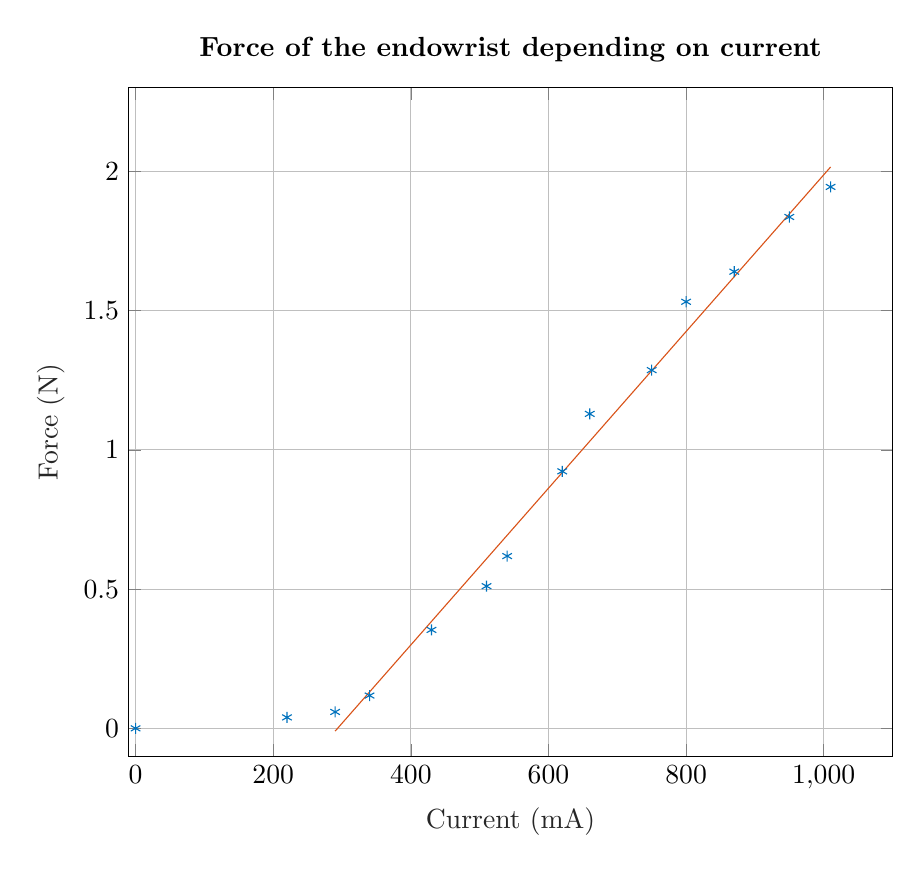
\begin{tikzpicture}

\begin{axis}[%
width=0.8\columnwidth,%7.484in,
height=0.7\columnwidth,%8.26in,
at={(0.758in,0.481in)},
scale only axis,
xmin=-10,
xmax=1100,
xlabel style={font=\color{white!15!black}},
xlabel={Current (mA)},
ymin=-0.1,
ymax=2.3,
ylabel style={font=\color{white!15!black}},
ylabel={Force (N)},
axis background/.style={fill=white},
title style={font=\bfseries},
title={Force of the endowrist depending on current},
xmajorgrids,
ymajorgrids
]
\addplot [color=mycolor1, draw=none, mark=asterisk, mark options={solid, mycolor1}, forget plot]
  table[row sep=crcr]{%
0	0\\
220	0.03928\\
290	0.05892\\
340	0.11784\\
430	0.35352\\
510	0.51064\\
540	0.61866\\
620	0.92308\\
660	1.1293\\
750	1.28642\\
800	1.53192\\
870	1.63994\\
950	1.83634\\
1010	1.94436\\
};
\addplot [color=mycolor2, forget plot]
  table[row sep=crcr]{%
290	-0.00996204344902341\\
340	0.130719594329395\\
430	0.383946542330548\\
510	0.609037162776017\\
540	0.693446145443068\\
620	0.918536765888537\\
660	1.03108207611127\\
750	1.28430902411242\\
800	1.42499066189084\\
870	1.62194495478063\\
950	1.8470355752261\\
1010	2.0158535405602\\
};
\end{axis}
\end{tikzpicture}%
\caption{The force measurements from the end-effector}
\label{endo_force_mes}
\end{figure}

\subsection*{Uncertainties of measurement:}
\begin{itemize}
\item Not 100 \% orthogonal force to the load cell.
\item Input/Output impedance of sensors have a $\pm 10 \%$ tolerance.
\item Movement of test setup when force is generated.
\end{itemize}

\subsection*{Conclusion:}
\todo{conclusion}